\documentclass[a4paper,12pt]{article}

\usepackage[utf8]{inputenc}
\usepackage[T1]{fontenc}
\usepackage{color}
\definecolor{grey}{rgb}{0.9,0.9,0.9}
\definecolor{teal}{rgb}{0.0,0.5,0.5}
\definecolor{violet}{rgb}{0.5,0,0.5}
\usepackage[margin=2.5cm]{geometry}

\title{TP1 - Apprentissage supervisé}
\author{\textsc{Paul Chaignon} - \textsc{Ulysse Goarant}}
\date{\today}

\begin{document}

\maketitle

\section{Apprentissage d'un SVM}

\subsection{Données linéairement séparables}

\subsubsection*{\'Etape 1}
% TODO Add reference to figure.
\begin{figure}
	\center
	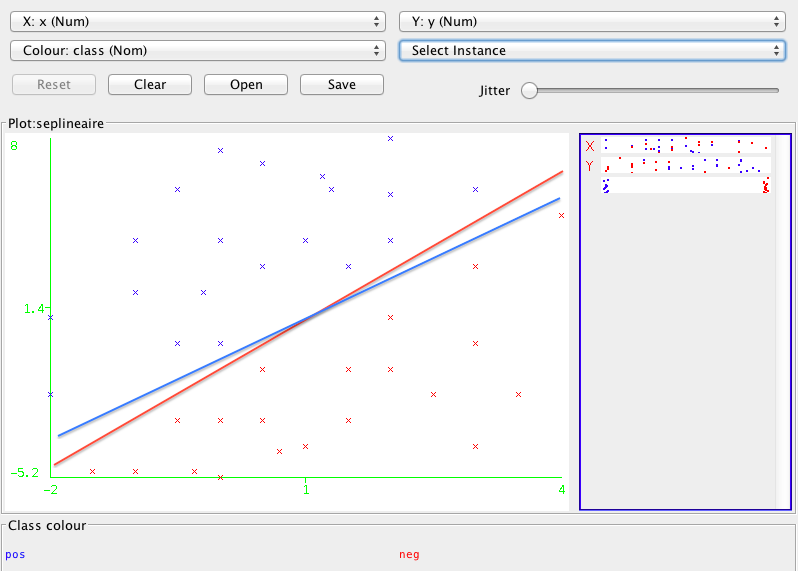
\includegraphics[width=1\textwidth]{SVM-graphe.png}
	\caption{Données linéairement séparables}
	\label{fig:svm-graphe}
\end{figure}
Les deux classes peuvent être séparées ici par une infinité de droites, ici deux possibles sont représentées.

\subsubsection*{\'Etape 2}
La droite optimale a pour équation : y = 1.77x – 0.88.
Le risque empirique est nul (tous les éléments appartenant à l’ensemble d’apprentissage sont bien classés).


\subsubsection*{\'Etape 3}
% TODO Add reference to figure.
\begin{figure}
	\center
	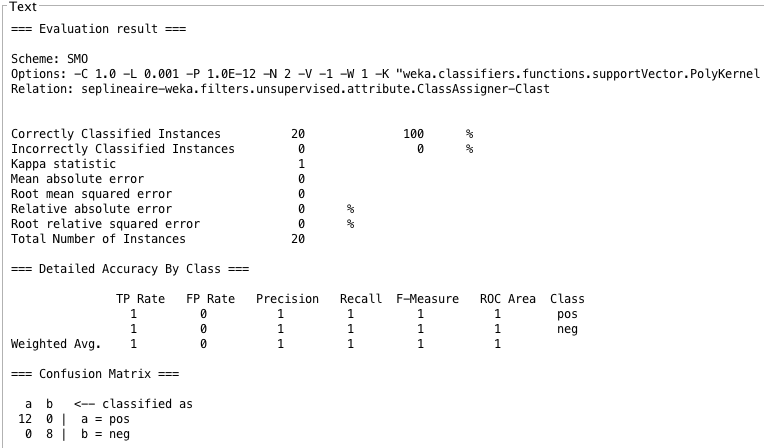
\includegraphics[width=1\textwidth]{SVM-table.png}
	\caption{Résultat de la méthode SMO sur les données linéairement séparables}
	\label{fig:svm-table}
\end{figure}
En séparant l’ensemble des exemples en un ensemble d’apprentissage (50\%) et un ensemble de test (50\%), le risque réel est nul.
Cependant, si l’on utilise seulement 10\% des données comme ensemble d’apprentissage, le risque réel croit à 55\%.


\subsection{Données non linéairement séparables}

% TODO Complete answer.
En utilisant un noyau Puk, il est possible de classer des exemples non linéairement indépendants.
Il y a dans ce cas 137 vecteurs de support impliqués.

\section{Apprentissage d'un arbre décision}


\subsection{Construction et évaluation d'arbres}

\subsubsection*{\'Etape 1}
Le fichier \textit{weather.nominal.arff} contient 14 instances.
Ils ont chacun 5 attributs dont 4 de type nominal et 1 de type booléen.
La classe à prédire est « play ».

\subsubsection*{\'Etape 2 & 3}
40\% des données de test ont bien été classées.
La matrice de confusion nous indique que le classement a été plus efficace à classer les \enquote{yes}.
% TODO Add reference to figure.
\begin{figure}
	\center
	\includegraphics[width=1\textwidth]{graphe-1.png}
	\caption{Arbre de décision J48}
	\label{fig:graphe-1}
\end{figure}

\subsubsection*{\'Etape 4}
En réduisant la part de l’ensemble des données d’apprentissage à 40\% et en modifiant la graine, le risque réel est réduit à 25\%.
% TODO Add reference to figure.
\begin{figure}
	\center
	\includegraphics[width=1\textwidth]{graphe-2.png}
	\caption{Amélioration de l'arbre de décision J48}
	\label{fig:graphe-2}
\end{figure}

\subsubsection*{\'Etape 5}
Ce nouveau jeu de données contient des attributs numériques.
L’arbre construit contient donc des nœuds testant des inégalités.

\section{\'Elagage et simplification}

% TODO Add reference to figure.
\begin{figure}
	\center
	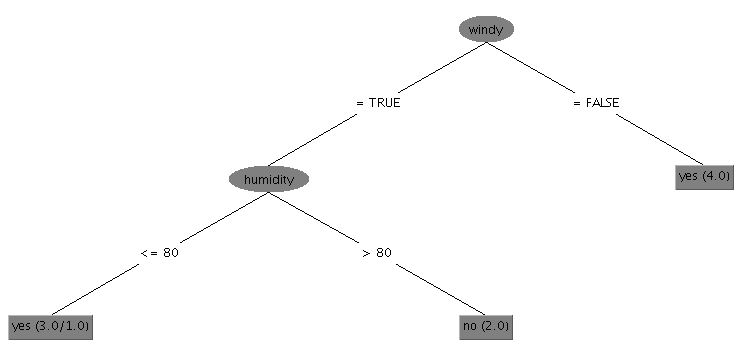
\includegraphics[width=1\textwidth]{arbre-elague.png}
	\caption{Arbre de décision élagué}
	\label{fig:arbre-elague}
\end{figure}
% TODO Add reference to figure.
\begin{figure}
	\center
	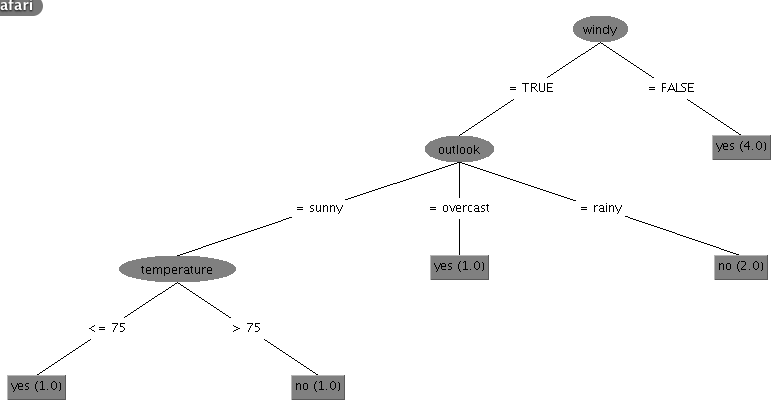
\includegraphics[width=1\textwidth]{arbre-non-elague.png}
	\caption{Arbre de décision non élagué}
	\label{fig:arbre-non-elague}
\end{figure}
L’arbre non-élagué obtient un meilleur taux de risque réel (40\%) comparé à l’arbre élagué (60\%), cependant le premier arbre a un plus grand risque d'avoir \enquote{coller aux données} que le second et a donc une capacité de généralisation moins forte.

\section{Apprentissage bayésien}


\subsection{Bayes naïf}

\subsubsection*{\'Etape 1}
L'hypothèse ici utilisée est que les attributs n'ont pas d'influence les uns sur les autres.

\subsubsection*{\'Etape 2}


\subsubsection*{\'Etape 3}


\subsubsection*{\'Etape 4}



\subsection{Approche non paramétrique}



\section{Fusion de classifieurs}



\end{document}